\documentclass[tikz,border=3pt]{standalone}
\usepackage[utf8]{inputenc}
\usepackage[T1]{fontenc}
\usepackage{lmodern}
\renewcommand{\familydefault}{\sfdefault}
\usepackage{sansmath}\sansmath
\usepackage{chemfig}
\usepackage{pgfplots}\pgfplotsset{compat=1.18,/pgf/number format/use comma,/pgf/number format/1000 sep={.}}
\usetikzlibrary{arrows.meta,calc,positioning,decorations.pathmorphing,patterns}
% paleta del sitio
\definecolor{nar}{HTML}{E8680C}\definecolor{narc}{HTML}{FFB35C}\definecolor{hielo}{HTML}{FFF3E8}
\definecolor{tinta}{HTML}{1D1D1F}\definecolor{gris}{HTML}{6E6E73}\definecolor{lila}{HTML}{7C5CF0}
\definecolor{azul}{HTML}{2F6FD6}\definecolor{menta}{HTML}{17A673}\definecolor{coral}{HTML}{E8342A}
\begin{document}
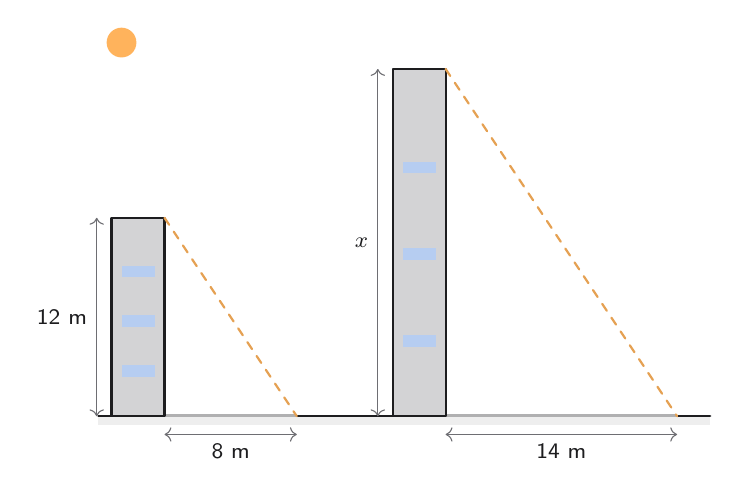
\begin{tikzpicture}[font=\small,x=0.42cm,y=0.42cm,line cap=round,line join=round,step={(1,1)}]
\fill[gris!12] (-2,-0.25) rectangle (16.5,0);
\draw[tinta,thick] (-2,0)--(16.5,0);
\fill[tinta!35] (0,-0.03) rectangle (4,0.08);
\filldraw[fill=gris!30,draw=tinta,thick] (-1.6,0) rectangle (0,6);\fill[azul!35] (-1.3,1.20) rectangle (-0.3,1.55);\fill[azul!35] (-1.3,2.70) rectangle (-0.3,3.05);\fill[azul!35] (-1.3,4.20) rectangle (-0.3,4.55);
\draw[narc!90!black,thick,dashed] (0,6)--(4,0);
\draw[<->,gris] (-2.0500000000000003,0)--(-2.0500000000000003,6) node[midway,left,font=\footnotesize,text=tinta] {12 m};
\draw[<->,gris] (0,-0.55)--(4,-0.55) node[midway,below,font=\footnotesize,text=tinta] {8 m};
\fill[tinta!35] (8.5,-0.03) rectangle (15.5,0.08);
\filldraw[fill=gris!30,draw=tinta,thick] (6.9,0) rectangle (8.5,10.5);\fill[azul!35] (7.2,2.10) rectangle (8.2,2.45);\fill[azul!35] (7.2,4.73) rectangle (8.2,5.08);\fill[azul!35] (7.2,7.35) rectangle (8.2,7.70);
\draw[narc!90!black,thick,dashed] (8.5,10.5)--(15.5,0);
\draw[<->,gris] (6.449999999999999,0)--(6.449999999999999,10.5) node[midway,left,font=\footnotesize,text=tinta] {$x$};
\draw[<->,gris] (8.5,-0.55)--(15.5,-0.55) node[midway,below,font=\footnotesize,text=tinta] {14 m};
\fill[narc] (-1.3,11.3) circle (0.45);
\end{tikzpicture}
\end{document}
